70. Построим параболу $y=x^2-4x-5$ по трём точкам $(5;0),\ (-1;0)$ и $(2;-9).$
$$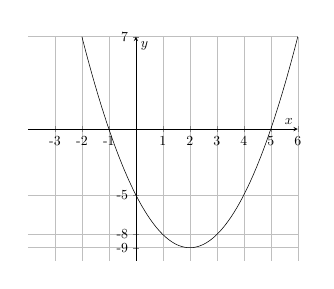
\begin{tikzpicture}[scale=0.5]
\begin{axis}[
    axis lines = middle,
    grid=major,
    legend pos={south west},
    xlabel = {$x$},
    ylabel = {$y$},
    ymin=-10,
    ymax=7,
    xmin=-4,
    xtick={-3,-1,1,3,5,2,-2,4,6},
    xticklabels={-3,-1,1,3,5,2,-2,4,6},
    ytick={ 7, -8, -5,-9},
    yticklabels={7, -8,-5,-9}           ]
	\addplot[domain=-2:6, samples=100, color=black] {x*x-4*x-5};
%\addplot[domain=-3:5, samples=100, color=black] {-abs(x-1)};
%\addplot[domain=-3.1:2.5, samples=100, color=red] {70*abs(1-2*abs(abs(x)-2))-10*x^2+10*x-70};
	%\addlegendentry{$\text{Рис. 1}$};
\end{axis}
\end{tikzpicture}$$
Исходя из графика, наименьшее значение функции на отрезке $[-1;3]$ равно $-9,$ а наибольшее --- 0.\\
